%% 
%% 
%% 

\chapter{Modeling Higer-order Structural Dependencies with Markov Random Fields (MRFs)}
\chaptermark{MRF-LSSVMs}
\label{cha:mrf}

One challenging task in machine learning is recognizing and
labeling over complex and structured objects. Many applications,
such as image segmentation, motif finding and noun-phrase
parsing, involves representing jointly correlated sub-objects and
exploiting structural dependencies to identify higher level
objects. These objects usually have structural dependencies on
sub-objects (smaller components), \eg the human face has a strong
structural dependency on five sensory organs. The Markov Random
Fields (MRFs, are also called undirected Probabilistic Graphical
Models~\cite{bishop:2006:PRML}), is one of the most popular
framework in modeling structural dependencies. In this Chapter,
we propose novel exact inference and learning algorithms, the
MRF-LSSVMs (Latent Structural Support Vector Machine) framework,
to exploit MRFs' capabilities in modeling higher-order (more than
three entities) structural dependencies. The application of
MRF-LSSVMs to capture higher-order dynamics on time series is
discussed in \Chapref{cha:mrf_lssvm_app}.

Markov Random Fields (MRFs) are undirected Probabilistic
Graphical Models (PGMs). The formulation of MRFs is simply a
regularized joint probability distribution. One specialty of MRFs
is that they are factorized (conditional independent) over
\textbf{maximal cliques} (more details in~\Secref{sec:MRF}) of
random variables defined on the undirected
graph~\cite{bishop:2006:PRML}. In many applications, structural
information, such as sub-objects to the whole object
relationships and relationships between sub-objects, can be well
represented in maximal cliques. By defining each maximal clique's
probability distribution and optimizing over them, MRFs provide a
powerful framework for modeling complex higher-order
dependencies between entities.

Utilizing MRFs usually involves three steps: 1) designing energy
functions (un-normalized probability distribution) according to
the actual problem, 2) solving inference problem (MAP or energy
minimization), and 3) learning parameters from data set. With
respect to energy functions, our work focuses on Lower Linear
Envelope Potentials (LLEP), a class of higher-order potentials
defined as a concave piecewise linear function over a clique of
random variables. LLEP has been raising much interest in the
image segmentation area, in which the raw image input is used as
PGM's graph and pixels are treated as random variables. Maximal
cliques of the input image are usually detected at preprocessing
stage by using clustering algorithms such as
superpixel~\cite{achanta2012slic}. Success of LLEP on encoding
consistent constraints over large subsets of pixels in image
segmentation tasks has been witnessed in many
literatures~\cite{Kohli:CVPR07,Nowozin:2011, Song2015}. In this
chapter we focus on proposing a novel exact inference algorithm
for LLEP and design a learning algorithm under the LLSVM
framework. In \Chapref{cha:mrf_lssvm_app}, we will generalize the
MRF-LLSVMs framework into encoding consistent constraints among
time-series' entities.

In the second step, in order to solve the inference problem of
LLEP, \citename{kohli2009robust} proposed a method to represent a
class of higher order potentials with lower (upper) linear
envelope potentials. By introducing auxiliary
variables~\cite{Kohli:CVPR10}, they reduced the linear
representation to a pairwise form and proposed an approximate
algorithm with standard linear programming methods. However, they
only show an exact inference algorithm on at most three terms.
Following their approach, \citename{gouldlearning} extended their
method to a weighted lower linear envelope with arbitrary many
terms solved with an efficient algorithm. They showed that the by
introducing auxiliary variables into LLEP, a quadratic
pseudo-Boolean form~\cite{Boros:MATH02} can be developed. This
psuedo-Boolean form is submodular and can be inferred efficiently
and exactly through graph-cuts like
algorithms~\cite{Boykov:ICCV01}. However, in order to employ
Structural Support Vector Machine (SSVM) to solve the learning
problem of LLEP, \citename{gouldlearning} have to sample the LLEP
using a set of fixed space points. Althought this formulation can
be globally optimized by using the SSVM framework, it lost a rich
class of representations of energy function due to the fixed
space sampling. In this chapter, we an alternative formulation to
learn LLEP exactly. We introduce auxiliary variables back to LLEP
and propose a graph-cuts algorithm to infer observed variables
and auxiliary variables simultaneously. Experiments in
~\Secref{sec:synth-check} also show that LLEP under this
formulation the algorithm can be learned exactly from various
different probability distribution configurations.

The third and last difficulty is to design a learning algorithm
for our LLEP formulation. In previous work,
\citename{gouldlearning} sampled the LLEP with fixed space points
and solved the learning problem under the Structural Support
Vector Machine (SSVM) framework \cite{tsochantaridis2005large}.
However, since we add auxiliary variables back, SSVM does not fit
our case anymore. One of our main contribution is that we prove
that auxiliary variables introduced in LLEP can be formulated as
latent variables in SSVM. With additional convex constraints
added to the SSVM object, our formulation results to the Latent
SSVM (LSSVM) framework \cite{yu2009learning}. The LSSVM was
developed by \citename{felzenszwalb2008discriminatively} and
\citename{yu2009learning} independently in different ways. The
main idea is introducing a latent variable to extend the feature
vector, which results in an arbitrary loss function, e.g. Hinge
Loss, with an upper bound. Then the optimization was done by
using Concave-Convex Procedure (CCCP) algorithm, which is
guaranteed to decrease the objective function to a local minimum.
In this thesis, we propose a variant formulation of
\cite{gouldlearning} by rewriting the lower linear envelope
function directly into a linear combination with latent feature
vectors and developing the learning algorithm using the LSSVM.

The rest of the thesis is structured as follows:
\Secref{sec:RelatedWorks} introduces background and related works
of MRFs and LSSVM. \Secref{sec:inference} proposes our first
contribution, the exact inference method of LLEP with auxiliary
variables. In~\Secref{sec:learning}, we reformulate the LLEP into
a linear combination and develop the learning algorithm under the
LSSVM framework. \Secref{sec:synth-check} conduct experiments on
a synthetic checkerboard image to show the effectiveness of our
novel MRF-LLSVMs framework. Application of MRF-LLSVMs on real
financial time-series data set is discussed in
\Chapref{cha:mrf_lssvm_app}.

\section{Background \& Related Works}
\label{sec:RelatedWorks}

\subsection{Markov Random Fields}
\label{sec:MRF}
From a PGMs view (\figref{fig:prml_mrf}) \cite{Bishop:2007},
MRFs' joint probability distribution can be represented as an
undirected graph and each random variable can be represented as a
node in the graph. A \textbf{clique} is a fully connected subset
of nodes: there exists a path between any pair of nodes in it. A
\textbf{maximal clique} is a clique such that it is not possible
to include any other nodes from the graph in the set without it
ceasing to be a clique.
\begin{figure}[ht]
  \centering
  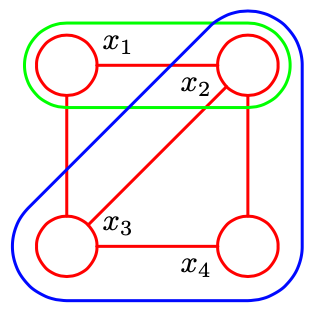
\includegraphics[width=0.3\columnwidth]{Part2/figures/prml_mrf}
  \caption{\label{fig:prml_mrf} An example PGM of MRFs. Each node
    in this graph corresponds to a random variable in this PGM's
    joint probability distribution. A clique is outlined in green
    circle and a maximal clique is outlined in blue circle.}
\end{figure}
Let $C$ denotes a maximal clique in one graph and $\vy_C$ denotes
the set of variables in that clique. Then the joint distribution
can be written as:
\begin{align}
  p(\vy)=\frac{1}{Z}\prod_{C}{\Psi_C(\vy_C)}
\end{align}
\noindent where $\Psi$ is called \emph{potential functions} which
can be defined as any non-negative functions and
$Z=\sum_{\vy}\prod_{C}{\Psi_C(\vy_C)}$ which is a normalization
constant. To infer labels which best explains input data set, we
can find the \emph{maximum a posteriori} (MAP) labels by solving
$\vy^*=\argmax_{\vy}p(\vy)$. However, potential functions are
restricted to be non-negative to ensure it is a probability
distribution.

In order to have more flexible representations of probability
distributions, by taking exponential of potential terms, MRFs can
be represented as a regularized joint log-probability
distribution of arbitrary non-negative functions over a set of
maximal cliques on the PGM graph~\cite{bishop:2006:PRML}. Thus
the joint distribution becomes:
\begin{align}
  p(\vy)=\frac{1}{Z}exp(-\sum_{C}{E_C(\vy_C)})
\end{align}
\noindent where $E$ is called \emph{energy functions} which can be
arbitrary functions. Therefore, \emph{maximum a posteriori}
problem is equivalent to \emph{energy minimization} problem,
which is also known as the \emph{inference} problem:
\begin{align}
  \vy^*=\argmax_{\vy}p(\vy)=\argmin_{\vy}(\sum_{C}{E_C(\vy_C)})
\end{align}

The \emph{inference} problem is computationally expensive. There
has been many sub-optimal algorithms such as max-product
algorithm \cite{Globerson:NIPS07} been proposed to solve the
general MRFs' inference problem. However, \citename{Boros:MATH02}
proved that for submodular energy functions, there exist
efficient algorithms based on graph cuts
\cite{Ishikawa:CVPR09,Kohli:TR08} and are guaranteed to converge
to the global optimum. In \Secref{sec:inference} we formulate the
MRFs with Lower Linear Envelope Potentials (LLEP) as
psuedo-boolean functions and devise a graph cut algorithm for
exact inference.

As for the \emph{learning} problem, conventionally, energy
functions can be decomposed into three weighted parts: nodes
$\gN$, edges $\gE$ and higher order cliques (any group which has
more than 3 fully connected nodes in it)
$\gC$~\cite{Szummer:ECCV08}. Each term has its own weights. Let
$\vw$ be the vector of parameters and $\phi$ be arbitrary feature
function, then the energy can be decomposed as a set linear
combinations of weights and feature vectors:

\begin{align}
  \label{eq:energyfunction_UPH}
  E(\vy;\vw)=\sum_{i\in \gN}{\vw_i^U\phi^U(\vy_i)}+
  \sum_{(i,j)\in \gE}{\vw_{ij}^P\phi^P(\vy_i,\vy_j)}+
  \sum_{\vy_C\in \gC}{\vw_C^H\phi^H(\vy_C)}
\end{align}

\noindent where $U$ denotes \emph{unary} terms, $P$ denotes
\emph{pairwise} terms and $H$ denotes \emph{higher order} terms
(when $|C|>2$ namely each clique contains more than two
variables).

A weight vector $\vw$ is more preferable if it gives the
ground-truth assignments $\vy_t$ less than or equal to energy
value than any other assignments $y$:

\begin{align}
E(y_t,w)\leq E(y,w)~ \text{,~}\forall y \neq y_t
\text{,~} y\in \sY
\end{align}

Thus the goal of \emph{learning} MRFs is to learn the parameter
vector $\vw^*$ which returns the lowest energy value for the
ground-truth labels $y_t$ relative to any other assignments
$y$~\cite{Szummer:ECCV08}:

\begin{align}
\vw^* = argmax_{\vw}(E(y_t,w)-E(y,w))~ \text{,~}\forall y \neq y_t
\text{,~} y\in \sY
\end{align}

Solving the learning problem of MRFs is also computationally
expensive. In this thesis, we employ the efficient Latent
Structural Support Vector Machines (LSSVMs) algorithm to solve
our MRFs.

\subsection{Latent Structural SVMs}
\label{sec:latent-struct-svms}

The Structural Support Vector Machines (SSVMs) (also called
max-margin
framework)~\cite{Taskar:ICML05,tsochantaridis2005large} is a
principled approach to learn weights of pairwise MRFs
\citename{Szummer:ECCV08,Gould:ICML2011}.
\citename{gouldlearning} extended this framework with additional
linear constraints to enforce concavity on the weights, thus
allowing them to be used to learn MRFs with lower linear envelope
potentials. However, because SSVM does not include latent
variables in its feature vector, such methods only approximately
learn higher-order functions. In this thesis, we propose an
algorithm to optimize the energy function exactly by introducing
auxiliary variables back into the feature vector and solving the
learning problem using the Latent Structural SVMs (LSSVMs)
framework~\cite{yu2009learning}. To include unobserved
information, \citename{yu2009learning} extended the joint feature
function in structural SVM with latent variables and re-wrote the
objective function of SSVM into a difference of two convex
functions. This formulation can be solved using the
Concave-Convex Procedure (CCCP)\cite{yuille2002concave} which is
two-stages algorithm that guarantee to convergence to a local
minimum.

Specifically, given an a linear combination of features vector
$\phi(\vx ,\vy) \in \sR^m$ and weights $\vtheta \in \sR^m$, and a
set of $n$ training examples $\{\vy_i\}_{i=1}^n$ max-margin
framework can be used to solve optimized solution $\vtheta^*$. To
include unobserved information in the model,
Yu\cite{yu2009learning} extended the joint feature
function\cite{tsochantaridis2005large} $\phi(\vx,\vy) $ with a
latent variable $\vh\in \mathcal{H}$ to $\phi(\vx,\vy,\vh) $. So
the inference problem becomes
\begin{align}
  \label{eq:latent_ssvm_linearcomb}
  f_\theta(x) = \argmax_{(\vy \times \vh) \in \sY
  \times \sH} \vtheta\cdot\phi(\vx,\vy,\vh)
\end{align}

Accordingly, the loss function can be extended as

$$
\Delta((\vy_i,\vh^*_i(\theta)),(\hat{\vy}_i(\vtheta),\hat{\vh}_i(\vtheta)))
$$

\noindent where

\begin{align}
  \label{eq:latentssvm_full_inf}
 (\hat{\vy}_i(\vtheta),\hat{\vh}_i(\vtheta))=\argmax_{(\vy
  \times \vh) \in \mathcal{Y} \times \mathcal{H}}
\theta\cdot\phi(\vx_i,\vy,\vh)
\end{align}

\begin{align}
  \label{eq:latentssvm_latent_inf}
  \vh^*_i(\theta) = \argmax_{\vh \in \mathcal{H}} \theta \cdot
  \phi(\vx_i,\vy_i,\vh)
\end{align}

The loss function under this formulation measures difference
between the inferred result pair $(\hat{\vy}_i(\theta),
\hat{\vh}_i(\theta))$ and the pair $(\vy_i(\theta),
\vh_i^*(\theta))$ which best explains the training data. However,
under this formulation the ``loss augmented inference'' used in
structural SVMs\cite{tsochantaridis2005large} to remove the
complexity cannot be performed due to the dependence of loss
function $\Delta$ on hidden variables $\vh^*_i(\theta)$.
\citename{yu2009learning} argued that in real world applications
hidden variables are usually intermediate results and are not
required as an output\cite{yu2009learning}. Therefore, the loss
function can only focus on the inferenced hidden variables
$\hat{\vh}_i(\theta)$ which leads to:

$$
\Delta((\vy_i,\vh^*_i(\theta)),(\hat{\vy}_i(\theta),\hat{\vh}_i(\theta)))
=
\Delta(\vy_i,\hat{\vy}_i(\theta),\hat{\vh}_i(\theta))
$$

Thus the upper bound used in standard structural
SVMs\cite{tsochantaridis2005large} can be extended to:

\begin{align}
  \nonumber\Delta((\vy_i,\vh^*_i(\theta)),(\hat{\vy}_i(\theta),\hat{\vh}_i(\theta)))
  &\leq \bigg(\max_{(\hat{\vy} \times \hat{\vh}) \in
    \mathcal{Y} \times \mathcal{H}}
    [\theta\cdot\Psi(\vx_i,\hat{\vy},\hat{\vh}) +
    \Delta(\vy_i,\hat{\vy},\hat{\vh})]\bigg)\\
  &-\max_{\vh \in \mathcal{H}} \theta \cdot
    \Psi(\vx_i,\vy_i,\vh)
\end{align}

Hence the optimization problem for Structural SVMs with latent
variables becomes

\begin{align}
\label{eq:latent_ssvm_object}
  \min_\theta\bigg(\frac{1}{2}\|\theta\|^2+
  C\sum_{i=1}^{n}\big(\max_{(\hat{\vy} \times
  \hat{\vh}) \in \mathcal{Y} \times \mathcal{H}}
  [\theta\cdot\Psi(\vx_i,\hat{\vy},\hat{\vh}) +
  \Delta(\vy_i,\hat{\vy},\hat{\vh})]\big)\bigg)\\
  -C\sum_{i=1}^{n}\big(\max_{\vh \in \mathcal{H}} \theta \cdot
  \Psi(\vx_i,\vy_i,\vh)\big)\nonumber
\end{align}

\noindent which is a difference of two convex functions. Problem
of this formulation can be solved using the Concave-Convex
Procedure (CCCP)\cite{yuille2002concave} which is guaranteed to
converge to a local minimum. \citename{yu2009learning} proposed a
two stages algorithm. In the first step the latent variable
$\vh_i^*$ which best explains training pair $(\vx_i, \vy_i)$ is
found by solving equation~\eqref{eq:latentssvm_latent_inf}. This
step is also called the ``latent variable completion'' problem.
In the second step $\vh_i^*$ is used as completely observed to
substitute $\vh$ in equation~\eqref{eq:latent_ssvm_object}.
Therefore, solving equation~\eqref{eq:latent_ssvm_object} is
equivalent to solve the standard structural SVM problem.

In contrast to SVM, the latent structural SVM only provides an
optimization framework and cannot be directly applied. In order
to use it, the inference algorithm, as well as the MRF feature
function, loss function, and latent variable completion
problem~\cite{yu2009learning} must first be specified. Our
implementation of these terms are described in
section~\ref{sec:opt}.

\section[MRFs with LLEPs]{Markov Random Fields (MRFs) with Lower
  Linear Envelope Potentials (LLEPs)}
\label{sec:inference}

Energy functions can be decomposed over nodes $\gN$, edges $\gE$
and higher order cliques $\cal C$~\cite{Szummer:ECCV08}. Let
$\vw$ be vector of parameters and $\psi$ be arbitrary feature
function, then the energy can be decomposed as a set of linear
combinations of weights and feature vectors:

\begin{align}
  \label{eq:energyfunction_UPH}
  E(\vy;\vw)&=\sum_{i\in \gN}{\vw_i^U\psi^U(\vy_i)}+ \notag\\
  & \sum_{(i,j)\in \gE}{\vw_{ij}^P\psi^P(\vy_i,\vy_j)}+
  \sum_{\vy_C\in \cal C}{\vw_C^H\psi^H(\vy_C)}
\end{align}

\noindent where $U$ denotes \emph{unary} terms, $P$ denotes
\emph{pairwise} terms, $H$ denotes \emph{higher order} terms. In
this section we mainly focus on one class of higher-order
potentials $\psi^H$ defined as a concave piecewise linear
function which is known as \emph{Lower Linear Envelope
  Potentials} (LLEP). 

LLEP has been studied extensively in Markov Random Fields area
for encouraging consistency over large
cliques~\cite{Kohli:CVPR07,Nowozin:2011,Gould:ICML2011}. In
\Secref{sec:llep}, we begin with developing standard Markov
Random Fields (MRFs) (equation~\eqref{eq:energyfunction_UPH})
with the LLEP as energy functions. We then show how to perform
exact inference under this formulation in
\Secref{sec:exact_inference}. The optimization algorithm for our
formulation will be discussed in \Secref{sec:learning}.

\subsection{Higher-order Energy Functions: Weighted Lower Linear
  Envelope Potentials (LLEP)}
\label{sec:llep}

Let $\cal C$ denotes the set of all maximal cliques
and $\vy_c=\{y_i |\text{\,for\,} i \in C_j\}$ denotes set of
binary random variables where $y_i\in \{0,1\}$ in clique $C_j$, a
weighted lower linear envelope potential over $\vy_c$ is defined
as the minimum over a set of $K$ linear functions as:
%
\begin{align}
  \psi^H_c\!(\vy_c) \, &= \min_{k=1, \ldots, K} \left\{ a_k W_{\!c}(\vy_c) + b_k \right\}.
  \label{eqn:potential2}
\end{align}
%
where $W_{\!c}(\vy_c) = \sum_{i \in c} w_i^c y_i$ with $w^c_i
\geq 0$ and $\sum_{i \in c} w^c_i = 1$ which are weights for each
clique. $(a_k, b_k) \in \sR^2$ are the linear function
parameters. We illustrate an example with four linear functions
in \figref{fig:concave}.

\begin{figure}[t]
  \centering
  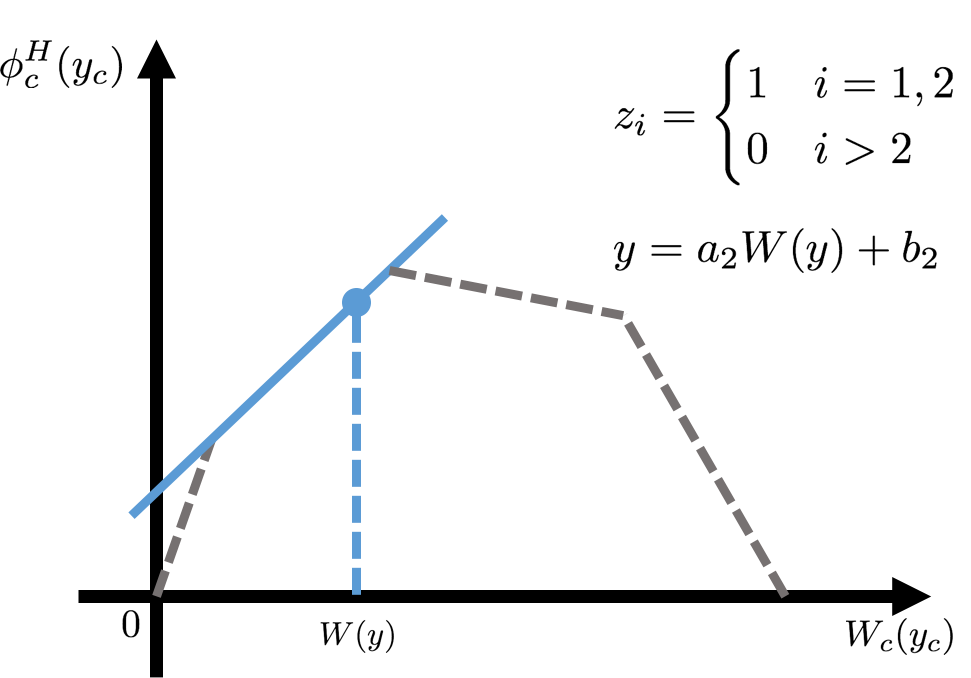
\includegraphics[width=0.8\columnwidth]{Part2/figures/linEnvLatentFig.png}
  \caption{\label{fig:concave} Example piecewise-linear concave
    function of $W_{\!c}(\vy_c) = \sum_{i \in c} w^c_i y_i$.
    Assume the second linear function is active namely
    $\vz^c=(1,1,0,0)$ (equation \ref{eqn:binary_concave_z}). The result of linear combination of
    parameter vector and feature vector is same as quadratic
    pseudo-Boolean function.}
\end{figure}

% % to_replace
% \begin{figure}[ht]
%   \centering
%   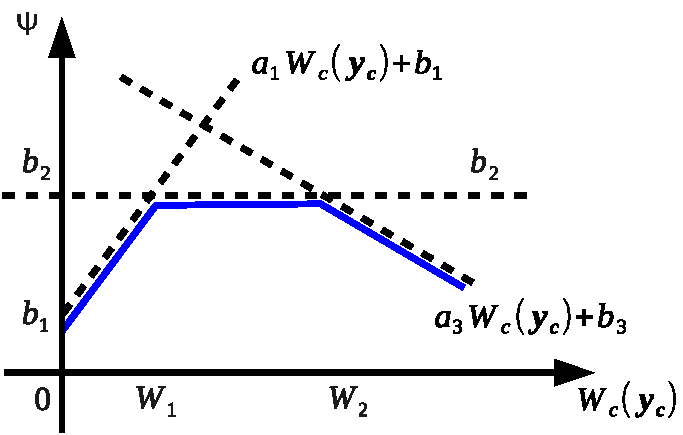
\includegraphics[width=0.6\columnwidth]{Part2/figures/not_redundant}
%   \caption{\label{fig:nonredundant} Example lower linear envelope
%     $\psi^H_c\!(\by_c)$ (shown solid) with three terms (dashed).
%     When $W_{\!c}(\by_c) \leq W_1$ the first linear function is
%     active, when $W_1 < W_{\!c}(\by_c) \leq W_2$ the second
%     linear function is active, otherwise the third linear
%     function is active.}
% \end{figure}

Inference on energy function contains lower linear potentials is
the same as the standard equation~\eqref{eq:energyfunction_UPH}
and is given by:
\begin{align}
  \label{eq:min_energy}
  \vy^* = \argmin\energy{\vy}
\end{align}

Suppose that parameters $\{(a_k, b_k)\}_{k=1}^K$ are sorted in
decreasing order of $a_k$. From \emph{Definition 3.1}
\cite{gouldlearning} we know that the $k$-th linear function is
said to be \emph{active} if there exists $x \in (0, 1)$ such that
the following two inequalities hold
\begin{align}
  a_{k-1} x + b_{k-1} &> a_k x + b_k \nonumber \\
  a_{k+1} x + b_{k+1} &> a_k x + b_k
  \label{eqn:nonred_in_ab}
\end{align}
%
The $k$-th linear function is said to be \emph{redundant}
(\emph{Definition 3.2}~\cite{gouldlearning}) if it is not active
for any assignment to $\vy_c$ in any clique $c \in \gC$ or is only
active whenever another linear function is also active.
Figure \ref{fig:redundant} depicts such conditions. As a
result, removing redundant functions from the potential does not
chang the energy function.


From section~\ref{sec:MRF} we have already introduced that an
\emph{energy function} may contain \emph{unary}, \emph{pairwise}
and \emph{higher-order} potentials (see
equation~\eqref{eq:energyfunction_UPH}). In this section we
mainly focus on one class of higher-order potentials $\phi^H$
defined as a concave piecewise linear function which is known as
\emph{lower linear envelope potentials}. This has been studied
extensively in Markov Random Fields area for encouraging
consistency over large
cliques~\cite{Kohli:CVPR07,Nowozin:2011,Gould:ICML2011}.

Let $\gC$ denotes the set of all maximal cliques in an image and
$\vy_c=\{y_i |\text{\,for\,} i \in c\}$ denotes set of random
variables in the clique $c$, a weighted lower linear envelope
potential~\cite{gouldlearning} over $\vy_c$ is defined as the
minimum over a set of $K$ linear functions as:
%
\begin{align}
  \psi^H_c\!(\vy_c) \, &= \min_{k=1, \ldots, K} \left\{ a_k W_{\!c}(\vy_c) + b_k \right\}.
  \label{eqn:potential2}
\end{align}
%
where $W_{\!c}(\vy_c) = \sum_{i \in c} w_i y_i$ with $w^c_i \geq
0$ and $\sum_{i \in c} w^c_i = 1$ which are weights for each
clique. $(a_k, b_k) \in \sR^2$ are the linear function
parameters. We illustrate an example~\cite{gouldlearning} with
three linear functions in \figref{fig:nonredundant}.
%
\begin{figure}[ht]
  \centering
  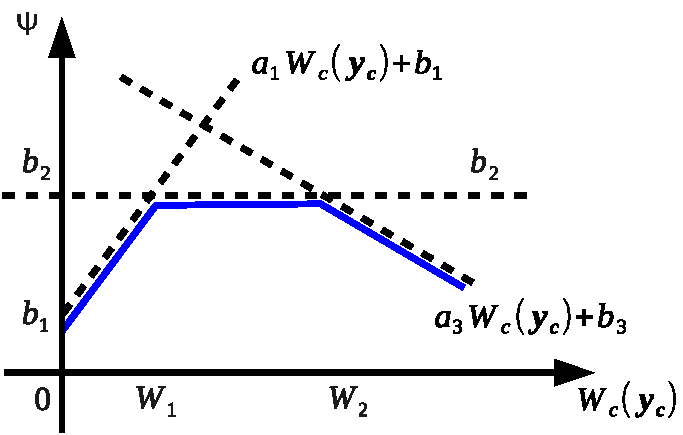
\includegraphics[width=0.6\columnwidth]{Part2/figures/not_redundant}
  \caption{\label{fig:nonredundant} Example lower linear envelope
    $\psi^H_c\!(\vy_c)$ (shown solid) with three terms (dashed).
    When $W_{\!c}(\vy_c) \leq W_1$ the first linear function is
    active, when $W_1 < W_{\!c}(\vy_c) \leq W_2$ the second
    linear function is active, otherwise the third linear
    function is active.}
\end{figure}

Suppose that parameters $\{(a_k, b_k)\}_{k=1}^K$ are sorted in
decreasing order of $a_k$. \citename{gouldlearning} (Definition
3.1) defines that the $k$-th linear function is said to be
\emph{active} if there exists $x \in (0, 1)$ such that the
following two inequalities hold
\begin{align}
  a_{k-1} x + b_{k-1} &> a_k x + b_k \nonumber \\
  a_{k+1} x + b_{k+1} &> a_k x + b_k
  \label{eqn:nonred_in_ab}
\end{align}
%
The $k$-th linear function is said to be \emph{redundant}
(\emph{Definition 3.2}~\cite{gouldlearning}) if it is not active
for any assignment to $\vy_c$ in any clique $c \in \gC$ or is only
active whenever another linear function is also active.
Figure \ref{fig:redundant} depicts such conditions. As a
result, removing redundant functions from the potential does not
chang the energy function.

\begin{figure}[ht]
  \centering
  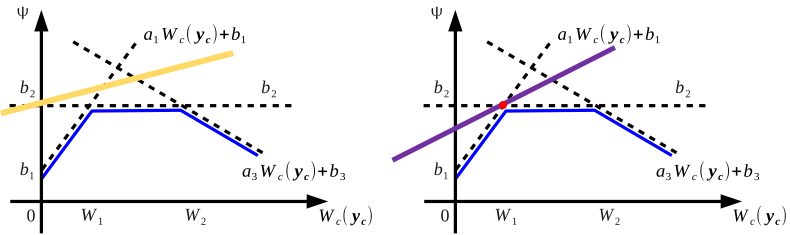
\includegraphics[width=1\columnwidth]{Part2/figures/redundant}
  \caption{\label{fig:redundant} Example lower linear envelope
    with redundant linear functions. On the left figure, the
    solid yellow line is always inactive. On the right figure,
    the solid purple line intersects $line \; 1$ and $line \; 2$
    at the red point. It's only active when $line \; 1$ and $line
    \; 2$ are both active. Both solid lines are redundant linear
    functions hence can be removed without changing their energy
    function.}
\end{figure}
%

To ensure potentials do not contain redundant linear functions
(functions that would never be active), \citename{gouldlearning}
proposed a constraint on parameters of the envelope. The $k$-th
linear function is not redundant if the following condition is
satisfied:
%
\begin{align}
    0
    <
    \frac{b_k - b_{k-1}}{a_{k-1} - a_k}
    <
    \frac{b_{k+1} - b_k}{a_k - a_{k+1}}
    <
    1.
  \label{eq:nonredundant}
\end{align}
%
Another important property of equation~\eqref{eq:min_energy} is
shift invariant (vertically). We write
$\widetilde{\psi}^{H}_c\!(\vy_c)$ by shift
equation~\eqref{eqn:potential2} vertically with an arbitrary
amount $b^{const}\in R$
$$\widetilde{\psi}^{H}_c\!(\vy_c) = \min_{k=1, \ldots, K}
\left\{a_k W_{\!c}(\vy_c) + b_k + b^\textrm{const} \right\}$$
%
Then we have
\begin{align}
  \argmin_{\vy_c} \psi^H_c\!(\vy_c)
  = \argmin_{\vy_c} \widetilde{\psi}^{H}_c\!(\vy_c).
  \label{eq:shift_invariant}
\end{align}
%
Therefore, in the following discussion without loss of generality
we assume $b_1 = 0$ thus $b_k\geq0 \text{\; for \;} k=1,\dots,n$.

\subsection{Exact Inference}
\label{sec:exact_inference}

Exact inference on MRFs has been extensively studied in past
years. Researchers found that, energy functions which can be
transformed into quadratic pseudo-Boolean
functions~\cite{Ishikawa:PAMI03,Ishikawa:CVPR09,Rother:CVPR09}
are able to be minimized exactly using \emph{graph-cuts} like
algorithms~\cite{Freedman:CVPR05,Hammer:1965} when they satisfy
submodularity condition~\cite{Boros:MATH02}.
\citename{Kohli:TR08} and \citename{Gould:ICML2011} adapted those
results to perform exact inference on lower linear envelope
potentials. In this section we mainly focus on describing the
minimum \emph{$st$-$cut$} graph constructed by
Gould~\cite{Gould:ICML2011,gouldlearning} for exact inference of
energy function (equation ~\eqref{eq:min_energy}) containing
lower linear envelope potentials.

Following the approach of \citename{Kohli:CVPR10},
\citename{Gould:ICML2011,gouldlearning} transformed the weighted
lower linear envelope potential in
equation~\eqref{eqn:potential2} into a quadratic pseudo-Boolean
function by introducing $K-1$ auxiliary variables $\vz =
\left(z_1, \ldots, z_{K-1}\right)$ with $z_k\in \{0,1\}$:

\begin{align}
  E^c(\vy_c, \vz) &= a_1 W_{\!c}(\vy_c) + b_1 \notag \\
  &+ \sum_{k = 1}^{K-1} z_k \left( \left(a_{k+1} - a_k\right) W_{\!c}(\vy_c) + b_{k+1} - b_k \right)
  \label{eqn:binary_concave_z}
\end{align}

\noindent for a single clique $c \in \cal C$. Under this
formulation, minimizing the pseudo-Boolean function over $\vz$ is
equivalent to selecting (one of) the active functions(s) from
equation~\eqref{eqn:potential2}. Another important property of
optimized $\vz$ under this formulation is that it automatically
satisfies the constraint
%
$$z_{k+1} \leq z_k$$
%
This property give rise to further development of parameter
vector and feature vector (equation~\eqref{eq:llsvm_param} and
~\eqref{eq:llsvm_feature}) which are used in latent structural
SVM. By introducing latent variables within the energy function,
we can learn richer energy representations than previous
study~\cite{gouldlearning} and solve inference problem exactly
within polynomial number of iterations.

In order to construct the minimum \emph{$st$-$cut$} graph, we
rewrite equation~\eqref{eqn:binary_concave_z} into
\emph{posiform}~\cite{Boros:MATH02}:

\begin{align}
  \label{eqn:posiform}  
  E^c(\vy_c, \vz)
  &= b_1 - (a_1 - a_K) + \sum_{i \in c} a_1 w^c_i y_i \notag\\
  & + \sum_{k = 1}^{K - 1} \left( b_{k+1} - b_k \right) z_k
    + \sum_{k = 1}^{K - 1} \left( a_k - a_{k+1} \right)
    \bar{z}_k\notag\\
  & + \sum_{k = 1}^{K - 1} \sum_{i \in c} \left( a_k - a_{k+1}
    \right) w^c_i \bar{y}_i z_k
\end{align}

\noindent where $\bar{z}_k = 1 - z_k$ and $\bar{y}_i = 1 - y_i$.
$a_1$ is assumed to be greater than $0$ so that all coefficients
are positive (recall we assume $b_1=0$ in section~\ref{sec:llep}
and we have $a_k > a_{k+1}$ and $b_k < b_{k+1}$). Since the energy function~\eqref{eqn:posiform}
is submodular, the \emph{st-min-cut} graph can be constructed 
based on equation~\eqref{eqn:posiform}.


\begin{figure}[t]
  \centering
  \setlength{\tabcolsep}{2pt}
  \begin{tabular}{cc}
    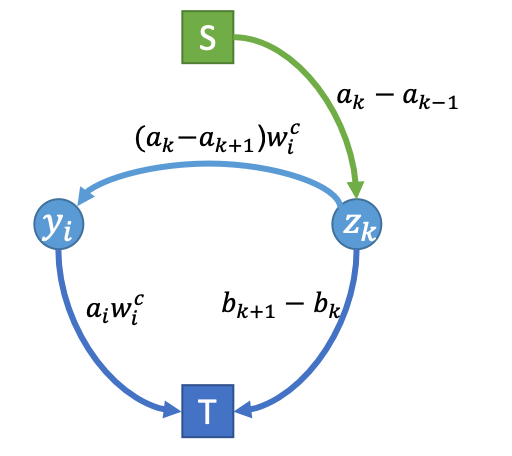
\includegraphics[width=0.47\columnwidth]{Part2/figures/ho.png}&
                                                                         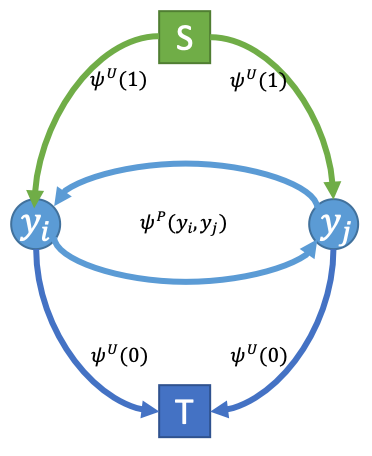
\includegraphics[width=0.37\columnwidth]{Part2/figures/up.png}\\
                                                                         {\small (a)} & {\small (b)} 
  \end{tabular}
  \caption{\label{fig:stmincut} $st$-graph construction for
    equation~\eqref{eqn:posiform}, unary and pairwise terms.
    Every cut corresponds to an assignment to the random
    variables, where variables associated with nodes in the $\gS$
    set take the value one, and those associated with nodes in
    the $\gT$ set take the value zero. With slight abuse of
    notation, we use the variables to denote nodes in our graph.}
\end{figure}


The construction (including unary and pairwise) is explained in
\Figref{fig:stmincut}. Figure (a) denotes construction for
equation~\eqref{eqn:posiform}. For each lower linear envelope
potential edges are added as follows: for each $i \in c$, add an
edge from $y_i$ to $t$ with weight $a_1 w^c_i$; for each $i \in
c$ and $k = 1, \ldots, K-1$, add an edge from $z_k$ to $y_i$ with
weight $(a_{k} - a_{k+1}) w^c_i$; and for $k = 1, \ldots, K-1$,
add an edge from $s$ to $z_k$ with weight $a_k - a_{k+1}$ and
edge from $z_k$ to $t$ with weight $b_{k+1} - b_k$. Figure (b)
denotes construction for unary and pairwise terms (see
\cite{Kolmogorov:PAMI04}). For unary edges (4 edges on both
sides), weights on each edge are corresponding to values in input
unary terms accordingly. For pairwise edges (2 edges in the
middle), both edges share the same weight which equals to the
input pairwise term.

\section[Solving MRFs under LSSVMs]{Solving MRFs under the Latent
  Structrual SVMs (LSSVM) Framework}
\label{sec:opt}

With the inference algorithm in hand, we now can develop the
learning algorithm for weighted lower linear envelope potentials
using the Latent Structural SVMs (LSSVMs) framework. In
\Secref{sec:learning}, we begin by transforming the
equation~\eqref{eqn:binary_concave_z} into a linear combination
of parameter vector and feature vector. A two-step algorithm was
developed to solve the latent structural SVM in
\Secref{sec:mrflssvm_learning_algo}.


\subsection{Transforming Between Representations}
\label{sec:learning}

The latent structural SVM formulation requires that the energy
function be formulated into a linear combination of features and
weights while our higher-order potential is represented as the
minimum over a set of linear functions. However,
in~\ref{sec:exact_inference} we reformulated the piesewise linear
functions into a quadratic pseudo-Boolean function in
equation~\eqref{eqn:binary_concave_z} by introducing auxiliary
variables. Now we show equation~\eqref{eqn:binary_concave_z}
itself is an inner product of parameter vector and feature vector
with latent information. Note that the function can be expanded
as a summation of $2K-1$ terms:

\begin{align}
  \label{eq:originalenergy}
  E^c(y_c,z)
  =&a_1W_c(y_c)+\sum_{k=1}^{K-1}(a_{k+1}-a_k)z_kW_c(y_c) \notag \\
   &+\sum_{k=1}^{K-1}(b_{k+1}-b_k)z_k
\end{align}

Here we use the fact of equation~\eqref{eq:shift_invariant} and
let $b_1=0$. Now we can reparameterize the energy function
as
\begin{align}
  \label{eq:llsvm_innerprod_energy}
  E^c(\vy_c,\vz; \vtheta^H) = \vtheta^{H^T} \! \psi^H(\vy_c,\vz)
\end{align}

\noindent where:

\begin{equation}
\label{eq:llsvm_param}
  \theta_k^H = \left\{
    \begin{aligned}
      & a_1	& \text{for} \ k=1\\
      & a_k-a_{k-1} & \text{for}\ 1< k \leq K\\
      & b_{k+1-K}-b_{k-K} & \text{for} \ K<k\le2K-1\\
    \end{aligned}
  \right.
\end{equation}

\begin{equation}
\label{eq:llsvm_feature}
  \psi_k^H = \left\{
		\begin{aligned}
      & W_c(\vy_c) 	& \text{for} \ k=1\\
      & W_c(\vy_c)\vz_k & \text{for}\ 1<k\le K\\
      & \vz_k & \text{for} \ K<k\le2K-1\\
		\end{aligned}
  \right.
\end{equation}

Under this formulation, similar to \cite{yu2009learning}, the inference problem
can be given by:

\begin{align}
  \label{eq:linenv_full_inf}
  (\mathbf{y}^*_k(\vtheta^H),\mathbf{z}^*_k(\theta^H))=\argmin_{(\mathbf{y}
  \times \mathbf{z}) \in \mathcal{Y} \times \mathcal{Z}}
  \vtheta^{H^T}\cdot\psi^H(\mathbf{y}_k,\mathbf{z}_k)
\end{align}
and
\begin{align}
  \label{eq:linenv_latent_inf}
  \mathbf{z}^*_k(\vtheta) = \argmin_{\mathbf{z} \in \mathcal{Z}}
  \vtheta^{H^T} \cdot \psi^H(\mathbf{y}_k,\mathbf{z}_k)
\end{align}

There are two facts worth to mention. The first fact is that in
our previous construction of minimum $st-cut$ graph the latent
variable $\vz$ is already included. Therefore, we can apply our
inference algorithm directly on our two new formulations. The
second fact is that for equation~\eqref{eq:linenv_latent_inf},
there exists a more efficient algorithm. At training stage, the
ground-truth labels $y_i$ is an input and is completely observed.
Therefore, the term $((a_{k+1}-a_k)W_c(\vy_c)+b_{k+1}-b_k)$ in
equation~\eqref{eq:originalenergy} becomes constant. So we can
infer latent variable $\vz$ explicitly by:
\begin{align}
  \label{eq:linenv_effi_infer_latent}
  z_k^c &=
          \begin{cases}
            0 & \text{if $((a_{k+1}-a_k)W_c(y_c)+b_{k+1}-b_k)\geq0$} \\
            1 & \text{otherwise}.
          \end{cases}
\end{align}

To show the equivalence between
equation~\eqref{eqn:binary_concave_z} and
equation~\eqref{eq:llsvm_innerprod_energy} we consider the
example illustrated in figure~\ref{fig:concave}. Assume the
inferred latent vector $\vz^c=(1,1,0,0)$. Plug it into
equation~\eqref{eq:llsvm_feature} the energy function can be
written as:
\begin{align*}
  E^c(\vy_c,\vz; \vtheta) &=
  \begin{bmatrix}
    a_1\\
    a_2-a_1\\
    a_3-a_2\\
    a_4-a_3\\
    b_2\\
    b_3-b_2\\
    b_4-b_3
  \end{bmatrix}^T
  \begin{bmatrix}
    W_c(\vy_c) \\
    W_c(\vy_c) \\
    0\\
    0\\
    1\\
    0\\
    0
  \end{bmatrix}\\
  &=a_1W_c(\vy_c)+(a_2-a_1)W_c(\vy_c)+b_2\\
  &=a_2W_c(\vy_c)+b_2
\end{align*}

Therefore, assignments inferred by graph-cut algorithm can be
directly encoded into a linear combination by using our latent
structural SVM formulation for learning purpose. The remaining
task is to ensure the concavity of $\vtheta$. We do this by
adding following constraint:

\begin{align}
  \label{eq:concave_constraint}
  A\vtheta\geq\epsilon \text{,\;~~~} A=
                  \begin{bmatrix}
                    1 & \mathbf{0} & \mathbf{0}\\
                    \mathbf{0} & -\mathbf{1} & \mathbf{0}\\
                    \mathbf{0} & \mathbf{0} & \mathbf{P}
                  \end{bmatrix}\in \mathbb{R}^{(2K-1)\times(2K-1)}
\end{align}

\noindent where $-\mathbf{1}$ is a matrix of size $(K-1)\times(K-1)$ and
$\mathbf{P}$ is an identity matrix of size $(K-1)\times(K-1)$.
One subtle problem we found during experiments is that the
algorithm can be stuck with small numerical value. To avoid this
we add small slack variables $\epsilon=\mathbf{1}^{-15}$ on 
those constraints.
\begin{align}
  \label{eq:concave_constraint}
  A\vtheta\geq\epsilon \text{,\;~~~} A=
                  \begin{bmatrix}
                    1 & \mathbf{0} & \mathbf{0}\\
                    \mathbf{0} & -\mathbf{1} & \mathbf{0}\\
                    \mathbf{0} & \mathbf{0} & \mathbf{P}
                  \end{bmatrix}\in \mathbb{R}^{(2K-1)\times(2K-1)}
\end{align}

\subsection{Latent Structural SVM Learning}
\label{sec:mrflssvm_learning_algo}

With the inner product formulation
(equation~\eqref{eq:llsvm_innerprod_energy}) of higher order
energy function, we are able to derive our latent
structural SVM learning algorithm. The energy function (higher
order function together with unary and pairwise functions) can be
written as:
\begin{equation}
  E_{all}(y,z) = \begin{bmatrix}
    \vtheta^H\\
    \theta^{unary}\\
    \theta^{pairwise}
  \end{bmatrix}^T 
  \cdot \begin{bmatrix}
    \psi^H\\
    \psi^{unary}\\
    \psi^{pairwise}
  \end{bmatrix}=\theta_{all}^T\cdot\psi_{all}
\end{equation}
where $\vtheta^H\in \sR^{2K-1}$ is the parameter vector in higher
order equation~\eqref{eq:llsvm_innerprod_energy} of size $2K-1$.
$\theta^{unary}$ and $\theta^{pairwise}$ are both scalars.
$\psi^\textrm{unary} = \sum_i \psi^U_i\!(y_i)$ and
$\psi^\textrm{pairwise} = \sum_{ij} \psi^P_{ij}(y_i, y_j)$.
Therefore, the size of $\theta_{all}$ is $2K+1$.

Plug equation~\eqref{eq:linenv_full_inf} and
equation~\eqref{eq:linenv_latent_inf} into object function in
\cite{yu2009learning}, the latent structural SVM object function
for our problem can be derived as a difference of two convex
functions:

\begin{align}
\label{eq:lssvm_object}
  \min_\theta\bigg(\frac{1}{2}\|\theta\|^2+
  C\sum_{i=1}^{n}\big(\max_{(\mathbf{\hat{y}} \times
  \mathbf{\hat{z}}) \in \mathcal{Y} \times \mathcal{Z}}
  [\theta\cdot\psi(\mathbf{\hat{y}},\mathbf{\hat{z}}) +
  \Delta(\mathbf{y}_i,\mathbf{\hat{y}},\mathbf{\hat{z}})]\big)\bigg)\\
  -C\sum_{i=1}^{n}\big(\max_{\mathbf{z} \in \mathcal{Z}} \theta \cdot
  \psi(\mathbf{y}_i,\mathbf{z})\big)\nonumber
\end{align}

Following \citename{yu2009learning}, we use the two stages
Concave-Convex Procedure (CCCP)~\cite{yuille2002concave} to solve
the optimization problem. We first imputes the latent variables
$\vz$ explicitly by equation~\eqref{eq:linenv_latent_inf}. Namely
solving the ``latent variable completion''
problem~\cite{yu2009learning}:

\begin{align}
  \vz_i^*=\argmax_{\mathbf{z} \in \mathcal{Z}} \theta \cdot
  \psi(\mathbf{y}_i,\mathbf{z})
\end{align}

The inference result $z_i^*$ for $i=1,\dots,n$ is used as
completely observed for later stage. With the latent variable
$z_i^*$ which best explains the ground-truth data $y_i$ in hand,
updating the parameter vector $\vtheta$ reduces to solve the
standard structural SVM problem:

\begin{align}
\label{eq:mrflssvm_object}
  \min_\theta\bigg(\frac{1}{2}\|\theta\|^2+
  C\sum_{i=1}^{n}\big(\max_{(\mathbf{\hat{y}} \times
  \mathbf{\hat{z}}) \in \mathcal{Y} \times \mathcal{Z}}
  [\theta\cdot\psi(\mathbf{\hat{y}},\mathbf{\hat{z}}) +
  \Delta(\mathbf{y}_i,\mathbf{\hat{y}},\mathbf{\hat{z}})]\big)\bigg)\\
  -C\sum_{i=1}^{n}\big(\theta \cdot
  \psi(\mathbf{y}_i,\mathbf{z}_i^*)\big) \nonumber
\end{align}

The last problem remaining is the initialization method. Because
our objective function~\eqref{eq:mrflssvm_object} is not convex
and the CCCP algorithm is only guaranteed to converge to a local
minimum or saddle point\cite{yuille2002concave}, initialization
of $\vtheta$ might affect the performance of our algorithm. Since
there are no theoretical solution for this problem, we propose an
empirical initialization algorithm in \Algref{alg:init_theta}.

\begin{algorithm}[ht]
  \begin{algorithmic}[1]
    \STATE{$gap=\frac{1}{K}$, $a_1=\sU(0,1e6)$, $b_1=0$,
      $sp_1=(0,0)$, $w_0=0$, $counter=2$} \FOR{each
      clique $c\in \gC$} \STATE{Compute weighted clique value
      $w_c=W_c(y_C)$} \IF{$w_c-w_{c-1}>gap$}
    \STATE{$upbound = a_{counter}w_c+b_{counter}$\\
      $sp_{counter}=(w_c,\sU(upbound-0.5,upbound))$\\
      Calculate $a_{counter}$ and $b_{counter}$ using
      $sp_{counter-1}$ and $sp_{counter}$\\
      $counter=counter+1$}
    \ENDIF
    \ENDFOR
    \STATE{If $counter<K$, remaining $a$s and $b$s are all set to
      be $a_{counter}$ and $b_{counter}$} \STATE{Calculate
      $\vtheta$ using $\{a_k,b_k\}_{k=1}^K$}
  \end{algorithmic}
  \caption{\label{alg:init_theta} Empirical initialization
    algorithm for $\vtheta$}
\end{algorithm}

We assume that the more evenly distributed of $W_c(Y_c)$ where
$c\in\gC$ on $x$ axis, the more rich representation (number of
linear functions) the energy function should have. In order to
initialize $\vtheta$, we first determine the x-coordinate of
sampled points $sp$. Then we sample its y-coordinate from a
uniform distribution $\sU(upbound,upbound-0.5)$ to add some
randomness in our initialization as well as maintain concavity.
Linear parameters $a_k$ and $b_k$ are later calculated using
those sampled points $sp_k$ and $sp_{k-1}$. At last we encode
$\{a_k,b_k\}_{k=1}^K$ into $\vtheta$ using
equation~\eqref{eq:llsvm_param}.

Our optimization algorithm is summarized in
\algref{alg:learning}.

\begin{algorithm}[hb]
  \begin{algorithmic}[1]
    \STATE{Set $MaxIter = 100$}
    \STATE{ {\bf input} training set $\{\vy_i\}_{i=1}^{n}$, regularization constant $C > 0$,
      and tolerance $\epsilon \geq 0$}
    \STATE{Initialize $\vtheta$ using \algref{alg:init_theta}}
    \REPEAT
    \STATE{Set $iter = 0$}
    \FOR{each training example, $i = 1, \ldots, n$}
    \STATE{compute $ \vz_i^*=\argmax_{\mathbf{z} \in \mathcal{Z}}
      \theta \cdot \phi(\mathbf{y}_i,\mathbf{z}) $}
    \ENDFOR

    \STATE{ {\bf initialize} active constraints set $\gC_i = \{ \}$ for all $i$}
    \REPEAT

    \STATE{solve the quadratic programming problem in
      equation~\ref{eq:mrflssvm_object} with respect to active
      constraints set $\gC_i$ for all $i$ and concavity constraints
      $A\vtheta\geq \epsilon$ to get
      $\hat{\vtheta}$ and $\hat{\vx_i}$}

    \FOR{each training example, $i = 1, \ldots, n$}
    \STATE{compute $\hat{\vy_i},\hat{\vz_i} = \argmin_{\vy}
      E(\vy,\vz; \hat{\vtheta}) - \Delta(\vy, \vz, \vy_i)$}
    \IF{$\hat{\xi}_i + \epsilon \!<\! \Delta(\hat{\vy_i},
      \hat{\vz_i}, \vy_i) -
      E(\hat{\vy_i},\hat{\vz_i}; \hat{\vtheta}) + E(\vy_i, \vz_i^*; \hat{\vtheta})$}
    \STATE{$\gC_i \leftarrow \gC_i \cup \{\vy_i^\star\}$}
    \ENDIF
    \ENDFOR
    \UNTIL{no more violated constraints}
    \STATE{ {\bf return} parameters $\hat{\vtheta}$}
    \STATE{Set $iter = iter+1$}

    \UNTIL{$iter\geq MaxIter$}
    \STATE{ {\bf return} parameters $\hat{\vtheta}$}
  \end{algorithmic}
  \caption{\label{alg:learning} Learning lower linear envelope
    MRFs with latent variables.}
\end{algorithm}

\section{Experiments}
\label{sec:synth-check}

Since the main contribution of our work is extending our previous
approximate formulation of lower linear envelope potentials to an
exactly formulation, it is necessary to compare the performance
of MRF-LLSVMs to previous work~\cite{gouldlearning}. In this
section, we examine our method's effectiveness by comparing our
results with~\cite{gouldlearning,Gould:ICML2011} on a synthetic
checkerboard. In order to demonstrate that our formulation has
the capability to learn a much richer class of energy function's
representation, we experiment our method on three different
problem instances: checkerboard with squares containing
monotonous color~\ref{sec:monot-color-squar}, checkerboard with
squares containing more pixels of one color over
another~\ref{sec:unbal-color-squar} and checkerboard with
uniformly colored squares containing unbalanced
color~\ref{sec:unif-distr-squar}.

\subsection{Experiment Settings}
\label{sec:experiment-settings}

An image of synthetic checkerboard contains $8 \times 8$ pixel
squares. Each square (clique) contains $16 \times 16$ (256)
pixels. The color of each pixel is either black $0$ or white $1$.
Given a ground-truth checkerboard image
$\vy^*=y^*_1,\dots,y^*_{16384}$, the observed unary terms
$\vy=y_1,\dots,y_{16384}$ are generated as followings. Let
$\eta_0$ and $\eta_1$ be the signal-to-noise ratios for the black
and white squares, the unary terms are generated by destroying
groud-truth label to noisy input
\begin{align}
  \label{eq:noisy_checkerboard}
  y_i = \eta_0 \ind{y^\star_i = 0} - \eta_1 \ind{y^\star_i = 1} + \delta_i
\end{align}
where $\delta_i
\sim \sU(-1, 1)$ is additive i.i.d.\ uniform noise. $\ind{x}$ is
an indicator function which equals $1$ when $x$ is true and $0$
otherwise. The task is to recover the ground-truth checkerboard
from the noisy input.

Our MRF is constructed on this image by associating each node in
the MRF to each pixel in the image. Thus our MRF contains $8
\times 8 \times 256 = 16,384$ variables. The energy function used
in this experiment follows equation~\eqref{eq:energyfunction_UPH}
without pairwise terms.

\begin{align}
  \label{eq:syncheck_energy}
  E(\vy;\vtheta)=\theta^U\sum_{i\in \gN}{\phi^U(\vy_i)}+
  \sum_{\vy_c\in \gC}{\phi^H(\vy_c,\vz_c;\vtheta^H)}
\end{align}
where $\phi^U(\vy_i)=\vy_i$ and $\theta^U$ is a scalar weight for
unary terms. $\phi^H(\vy_c,\vz_c;\vtheta^H)=\vtheta^{H\;T} \!
\phi(\vy_c,\vz_c)$ is equivalent to
equation~\eqref{eq:llsvm_innerprod_energy} and added for each
square (clique $c$) in the checkerboard. The number of linear
equations $K$ in equation~\eqref{eq:llsvm_param} is set to be
$10$. The parameters $\theta^U$ and $\vtheta^H$ are learned using
\algref{alg:learning} with $MaxIter=100$. 

\subsection{Monotonous Colored Squares}
\label{sec:monot-color-squar}

\begin{figure}[hb]
  \centering
  \setlength{\tabcolsep}{2pt}
  \begin{tabular}{cc}
    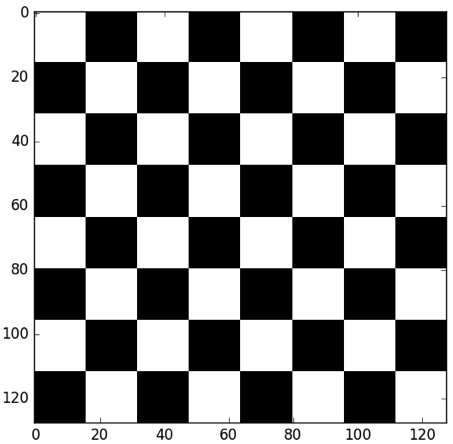
\includegraphics[width=0.5\columnwidth]{Part2/figures/mono_gt.png}&
                                                                            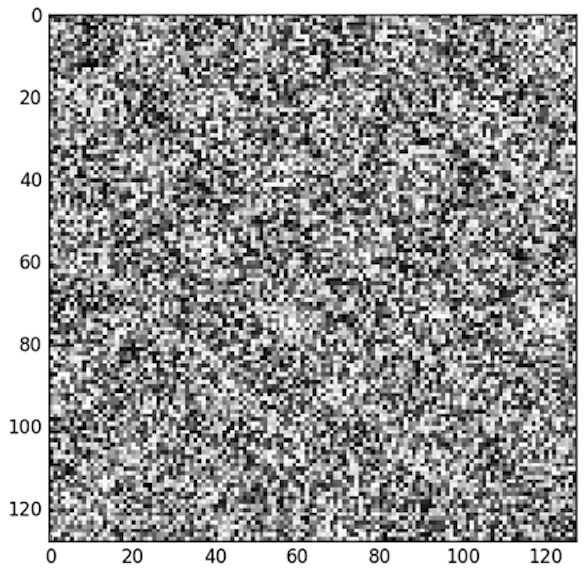
\includegraphics[width=0.5\columnwidth]{Part2/figures/mono_noisy.png}\\
    {\small (a)} & {\small (b)} 
  \end{tabular}
  \caption{\label{fig:mono_checkerboard} Example for monotonous
    colored squares. figure (a) is the ground-truth checkerboard.
    Figure (b) is the noisy input (unary terms) destroyed by
    equation~\eqref{eq:noisy_checkerboard}}
\end{figure}

We first repeat our previous black and white checkerboard
experiment~\cite{Gould:ICML2011,gouldlearning} in order to
examine the correctness of our new formulation. Each clique
(square) $c\in \gC$ in the checkerboard contains either all white
pixels $y_i=1 ,\;\forall i \in c$ or all black pixels $y_i=0
,\;\forall i \in c$. Figure~\ref{fig:mono_checkerboard}
illustrates the ground-truth checkerboard and the noisy input
destroyed by equation~\eqref{eq:noisy_checkerboard} with
$\eta_0=\eta_1=0.1$. Figure~\ref{fig:mono_results} shows the
results of our new method (on the bottom) together with our
previous method~\cite{gouldlearning} (on the top).

\begin{figure}[ht]
  \centering
  \setlength{\tabcolsep}{2pt}
  \begin{tabular}{cc}
    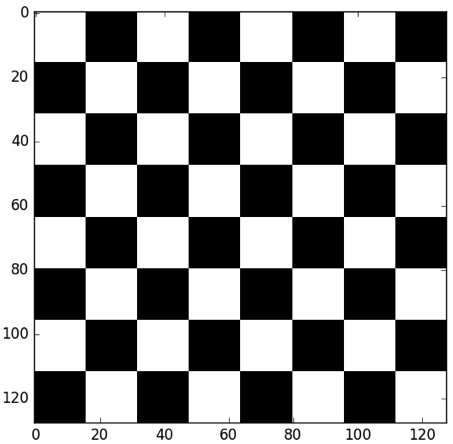
\includegraphics[width=0.3\columnwidth]{Part2/figures/mono_gt.png}&
                                                                              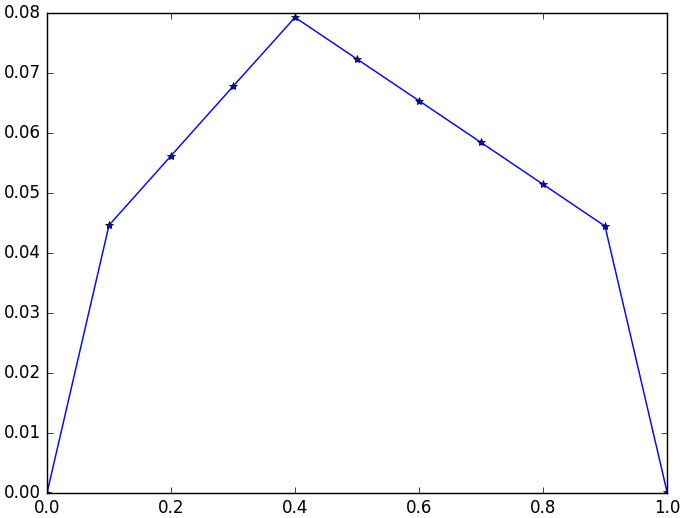
\includegraphics[width=0.4\columnwidth]{Part2/figures/mono_old.png}\\
    {\small (a)} & {\small (b)} \\
    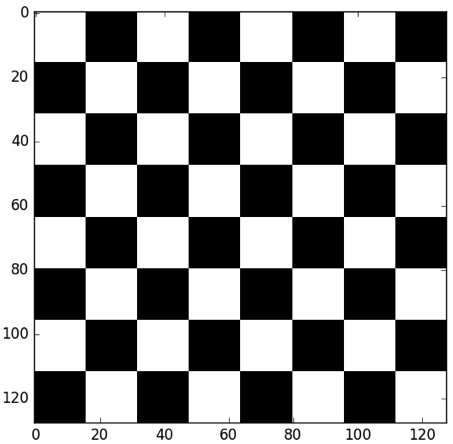
\includegraphics[width=0.3\columnwidth]{Part2/figures/mono_gt.png}&
                                                                              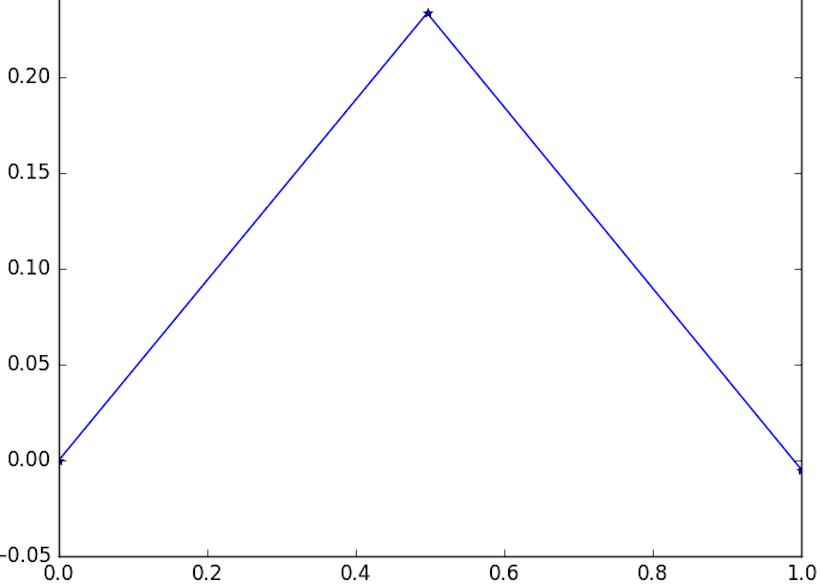
\includegraphics[width=0.4\columnwidth]{Part2/figures/mono_new.png}\\
    {\small (c)} & {\small (d)} 
  \end{tabular}
  \caption{\label{fig:mono_results} Results comparison for
    monotonous colored squares. Figure (a) and Figure (c) are
    inferred checkerboard from our previous and current
    formulation separately. Figure (b) and Figure (d) are lower
    linear envelopes learned by each formulation.}
\end{figure}

From figure~\ref{fig:mono_results} we conclude that both
formulations can recover checkerboard perfectly so our new
formulation's accuracy is as good as previous one. However,
there are significant differences between structural SVM
formulation (previous method) and latent structural SVM
formulation. There are $10$ active linear functions in
figure~\ref{fig:mono_results} (b) while there are only $2$ active
linear functions in figure~\ref{fig:mono_results} (d). Shapes
learned by each formulation are also significantly different.

In general, the second result is more preferable than the first
one. The reason is despite the image contains 64 cliques, there
are only two kinds of squares in the image: completely black and
completely white. Accordingly, our model only see two kinds of
cliques: completely $0$s (black) and completely $1$s (white). In
this case, a lower linear envelope contains two linear functions
is enough for encoding consistency information. This is reflected
in figure~\ref{fig:mono_results} (d) which gives least penalty
(0) when the clique value $W_C(y_c)$ equals either $0$ or $1$. It
gives the highest penalty when $W_C(y_c)$ is in the middle
because our model has least probability seen that in training
data. The results certificates that our latent structural SVM
formulation can learn lower linear envelope exactly. Therefore,
we say that our new method learns more preferable lower linear
envelope.

In terms of computational performance, because our initial point
are generated randomly using \algref{alg:init_theta}, the
performance various between runnings. On average it takes 2
\emph{outer loops} and 47 \emph{inner loops} to converge. Which
means the latent structural SVM formulation spends $3.5$ times
iterations to converge than previous one ($27$ iterations).
Each \emph{inner loop} took under 1s with inference taking about
120ms on a $2.7$GHz dual-core Intel CPU, which is the same as our
previous method.



\subsection{Unbalanced Colored Squares}
\label{sec:unbal-color-squar}

Experiment in section~\ref{sec:monot-color-squar} proves that our
latent structural SVM formulation can learn the lower linear
envelope exactly. In this section we conduct further experiment
to investigate its capability of representing unbalanced input.
The desirable result of this experiment should be the shape of
the lower linear envelope shifting along with the changing of
input data.

We design our checkerboards contain unbalanced colored squares as
shown in figure~\ref{fig:unba_checkerboard}.

\begin{figure}[hb]
  \centering
  \setlength{\tabcolsep}{2pt}
  \begin{tabular}{cc}
    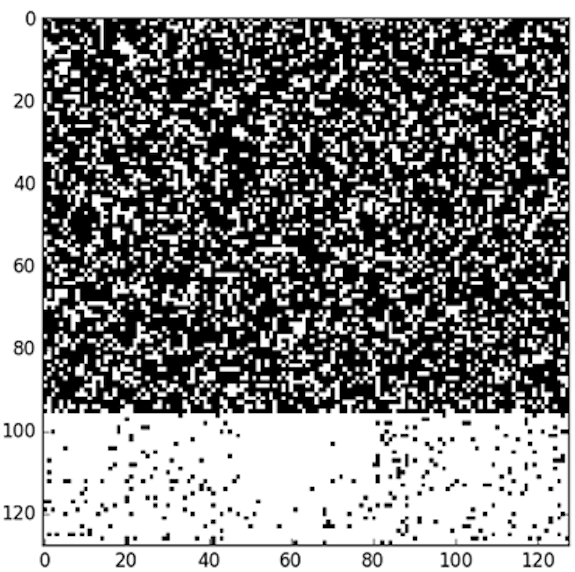
\includegraphics[width=0.5\columnwidth]{Part2/figures/unba_black.png}&
                                                                            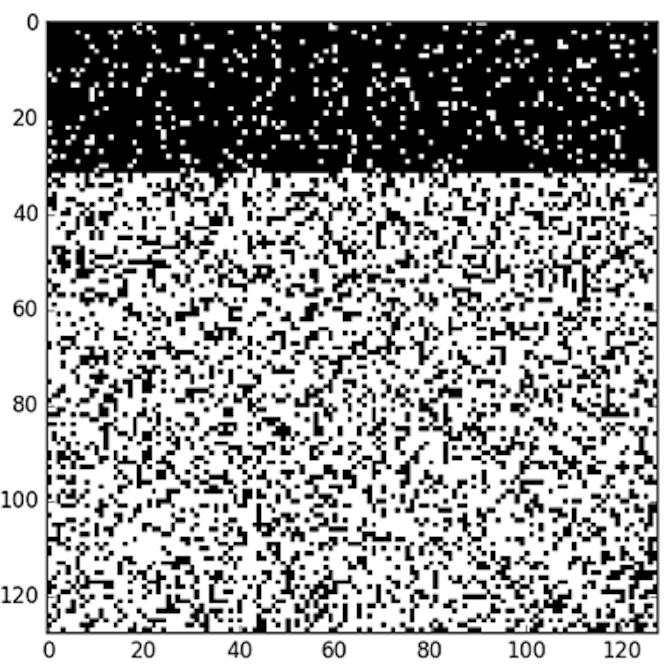
\includegraphics[width=0.5\columnwidth]{Part2/figures/unba_white.png}\\
    {\small (a)} & {\small (b)} 
  \end{tabular}
  \caption{\label{fig:unba_checkerboard} Example for unbalanced
    colored squares. In figure (a) $75\%$ cliques contain more
    than $85\%$ black pixels while $25\%$ cliques contain more
    than $85\%$ white pixels. Figure (b) is the opposite of
    figure (a)}
\end{figure}

As before, figure~\ref{fig:unba_results} shows results learned by
structural SVM (top row) and latent structural SVM (bottom row).
The accuracy performance of both methods are almost the same.
Both methods are able to recover $45\%-50\%$ pixels. The shape of
each formulations' results are both preferable and very similar
when compared to each other. The most significant difference is
the number of linear functions (10 active linear functions v.s.
2). In terms of computational performance, our previous method
only takes $10$ iterations to converge while the latent
structural SVM formulation takes $89$ iterations. Our new method
is much more computational expensive than our previous method.

\begin{figure}[ht]
  \centering
  \setlength{\tabcolsep}{2pt}
  \begin{tabular}{cc}
    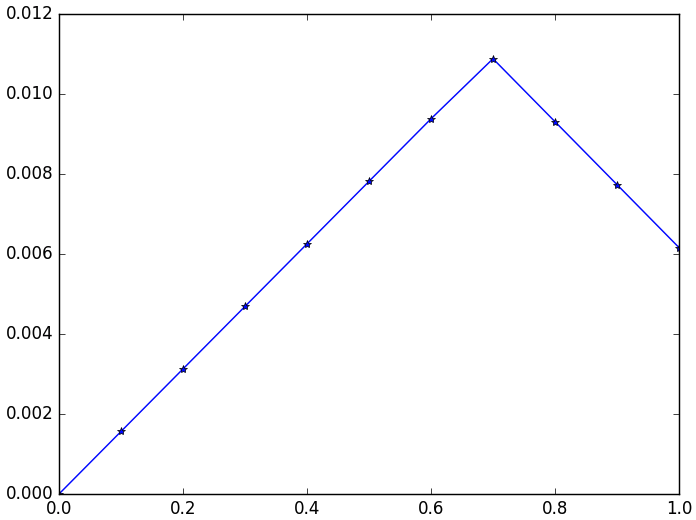
\includegraphics[width=0.5\columnwidth]{Part2/figures/unba_black_res_old.png}&
                                                                              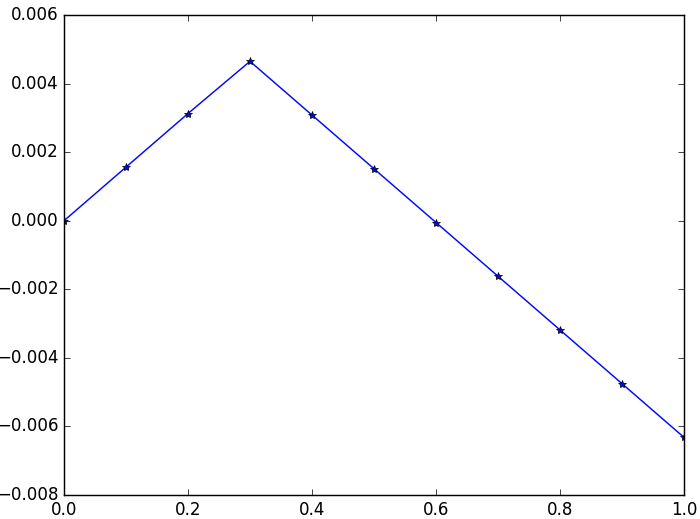
\includegraphics[width=0.5\columnwidth]{Part2/figures/unba_white_res_old.png}\\
    {\small (a)} & {\small (b)} \\
    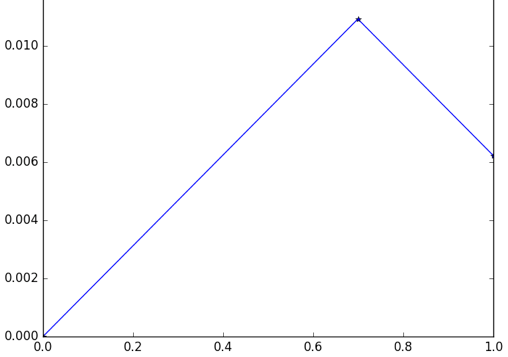
\includegraphics[width=0.5\columnwidth]{Part2/figures/unba_black_res_new.png}&
                                                                              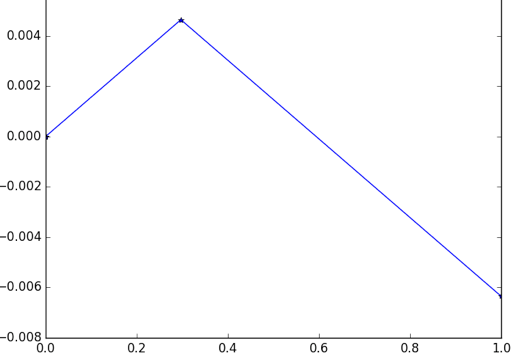
\includegraphics[width=0.5\columnwidth]{Part2/figures/unba_white_res_new.png}\\
    {\small (c)} & {\small (d)} 
  \end{tabular}
  \caption{\label{fig:unba_results} Results comparison for
    unbalanced colored squares. Figure (a) and Figure (b) are
    lower linear (more black and more white) envelopes learned by
    structural SVM. Figure (c) and Figure (d) are learned by
    latent structural SVM.}
\end{figure}

\subsection{Uniformly Colored Squares}
\label{sec:unif-distr-squar}

All of the above experiments show that our new method can
significantly simplify the shape of the lower linear envelope
function while maintaining the inference performance at the same
level. However, one significant cost is the computational
performance. It still remains obscure if there exists any other
advantages. In this section we design a much harder problem.
$W_c(y_c)$ is uniformly distributed from $0$ to $1$.
Figure~\ref{fig:ba_gt} shows the result. The preferable shape of
the lower linear envelope should contain a line which is parallel
to the x-axis.

\begin{figure}[t]
  \centering
  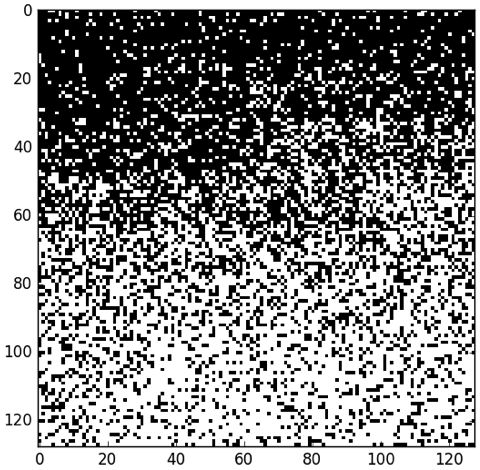
\includegraphics[width=0.5\columnwidth]{Part2/figures/ba_gt.png}
  \caption{\label{fig:ba_gt} Uniformly colored squares example.
    $W_{\!c}(\vy_c) = \sum_{i \in c} w^c_i y_i$ is uniformly
    distributed from $0$ to $1$.}
\end{figure}

Results are shown in figure~\ref{fig:ba_res}. As we can see
that shapes are very different between two formulations. Our
latent structural formulation (figure~\ref{fig:ba_res} (b))
learned a very flat representation of the lower linear envelope
function, which is much preferable, while the structural SVM
formulation preserves much concavity in the shape. This might
because in previous work~\cite{gouldlearning,Gould:ICML2011}
we imposed strict concave constraints on parameter vector
$\vtheta$.

The performance of accuracy also various significantly. Under
this formulation our new method is still able to recover
$45\%-50\%$ pixels while our previous can only recover
$25\%-30\%$ pixels on average. Therefore, our new formulation
finally outperforms previous one. In terms of computational
performance, the new formulation takes $129$ \emph{inner loops}
in total (2 \emph{outer loops}) while our previous formulation
takes $75$ iterations to converge. Although the new formulation
is still more computational expensive than previous one, the gap
decreases significantly.

We consider all of those improvements are due to our new method
is able to learn the lower linear envelope exactly.

One subtle thing is that the linear function on the right side in
figure~\ref{fig:ba_res} (b) decreases sharply which seems
abnormally at first glance. The reason is that we assume $b_1=0$
in section~\ref{sec:llep} which fixes the y-intercept of the
first linear function to be zero. Therefore the last linear
function can be arbitrarily deep while the first linear function
is fixed at the original point.

\begin{figure}[h]
  \centering
  \setlength{\tabcolsep}{2pt}
  \begin{tabular}{cc}
    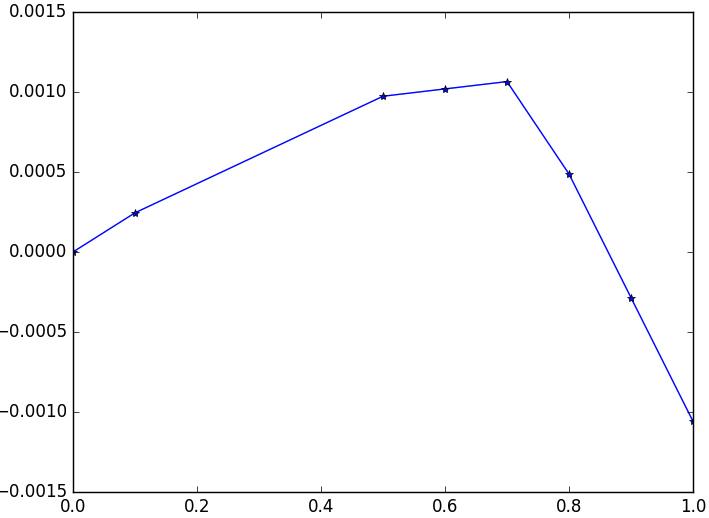
\includegraphics[width=0.5\columnwidth]{Part2/figures/ba_res_old.png}&
                                                                            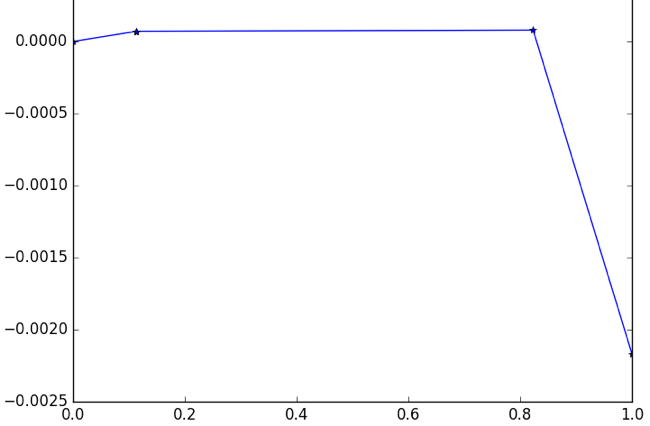
\includegraphics[width=0.55\columnwidth]{Part2/figures/ba_res_new.png}\\
    {\small (a)} & {\small (b)} 
  \end{tabular}
  \caption{\label{fig:ba_res} Results of uniformly colored
    squares experiment. Figure (a) is the result learned by
    structural SVM formulation. Figure (b) is the result learned
    by latent structural SVM formulation.}
\end{figure}

\subsection{Conclusions}
\label{sec:synth-check-conc}

From above experiments we conclude our findings as followings:

\begin{itemize}
\item All of those experiments verified that our latent
  structural formulation is able learn the lower linear envelope
  exactly.
\item In general (see section~\ref{sec:monot-color-squar} and
  section~\ref{sec:unbal-color-squar}), our new method have
  equivalent accuracy performance to our old method (structural
  SVM formulation\cite{Gould:ICML2011,gouldlearning}).
\item In terms of computational performance, the new formulation

  during training. However, it is more efficient during testing
  due to it simplicity for the lower linear envelope potentials.
\item For harder problem (see
  section~\ref{sec:unif-distr-squar}), the new method outperforms
  the previous one significantly. The gap of computational
  performance also decreases a significant amount.
\end{itemize}

%%% Local Variables:
%%% mode: latex
%%% TeX-master: "../thesis"
%%% End:
